\chapter{Algoritmo Propuesto}
\label{sec:modeloOpti}
%dado que se tienen muchos filamentos, se debe evaluar cual es mejor. Explicar como propiedades topológicas y geométricas tienen. Y como se ponderan para un peso que será minimizado o maximizado

En base a lo recopilado en los cap\'itulos previos de esta investigaci\'on, es posible destacar los siguientes aspectos del problema a resolver:

\begin{itemize}
    \item Se desconoce a priori el n\'umero de filamentos a buscar, dado que una imagen puede tener individualizaciones distintas para 2 expertos.
    \item Generalmente se busca individualizar m\'as de un filamento por imagen, lo que conlleva a elegir los mejores filamentos entre las soluciones que se encuentren.
    \item El uso de un grafo para representar la red de filamentos puede implicar que las combinaciones de soluciones crezcan de manera exponencial.
\end{itemize}

Lo anterior implica que el problema de identificar filamentos a partir de un grafo puede ser clasificado como un problema de optimizaci\'on con restricciones \cite{blum2011hybrid}.

Un problema de optimización con restricciones, (COP, Constrained Optimization Problem) puede ser representado como $P = (S, \Omega, F)$, donde S es el espacio de soluciones, $\Omega$ son las restricciones, y $F$ es la funci\'on objetivo. S esta definido por un conjunto discreto de variables $X = 1 \dotsc n$, con valores $v_{i}^{j} \in D_{i} = \{v_{i}^{1} \dotsc  v_{i}^{|D_{i}|}\}$. Se define como una variable {\it instanciada} la asignaci\'on a $X_i$ de un valor $v_{i}^{j} \in D_i$. Una solución candidata $s \in S$ es una soluci\'on factible si satisface las restricciones del conjunto $\Omega$. La funci\'on objetivo $F: S\rightarrow \mathbb R_{0}^{+}$, es la funci\'on de evaluaci\'on que asigna una puntuaci\'on a las soluciones candidatas. Al mismo tiempo, se define $s^{*}$ como una soluci\'on \'optima y $S^{*}$ como el conjunto que engloba todas las soluciones \'optimas, dado que pueden existir m\'ultiples soluciones $s^{*}$, y se relacionan mediante $s^{*} \in S^{*} \subseteq S $ \cite{socha2008ant}.
%Esta definici\'on permite aplicar la metaheur\'istica de optimizaci\'on basada en colonia de hormigas (ACO por su sigla en ingl\'es) a un modelo de un {\it COP}.
%COP es un CSP con función objetivo: https://en.wikipedia.org/wiki/Constrained_optimization#Constraint_optimization_problems

\section{Metaheur\'istica ACO}
\label{sec:hormigas}
La metaheur\'istica {\it Ant Colony Optimization} (ACO) se inspira en el comportamiento de una colonia de hormigas en la b\'usqueda del trayecto m\'as corto a una fuente de alimento, comunic\'andose entre ellas mediante feromonas. El recorrido de una hormiga se define como un camino $s$ y representa una soluci\'on en la b\'usqueda del camino m\'as corto.

Las hormigas realizan una exploraci\'on aleatoria alrededor de su hormiguero en busca de alimento. Una vez que lo encuentran, marcan el camino de retorno depositando una cantidad de feromonas, la que varia dependiendo de la calidad del camino. Para caminos de buena calidad, que son los de menor distancia entre un hormiguero y una fuente de alimento, las feromonas sirven de guía para otras hormigas. As\'i, las hormigas se comunican de forma indirecta, convergiendo en los caminos que tienen una mayor cantidad de feromonas. Este comportamiento se define como el modelo de feromonas y se observa en la Figura \ref{fig:hormigas}.


En este modelo, se define un camino como una soluci\'on $s$ que consiste en un conjunto de componentes de soluci\'on $c_{i}$, por lo que una concatenaci\'on de componentes de soluci\'on forma el camino o {\it tour} que recorre una hormiga. Cada componente $c_{i}$ tiene asociado un valor de feromona $\tau_i$, la cual influye en la elecci\'on que realiza una hormiga en relaci\'on a el o los componentes de soluci\'on disponibles para avanzar durante la construcci\'on de un camino. La metaheur\'istica ACO permite encontrar una \'unica soluci\'on o un conjunto de soluciones. 


\begin{figure}[h]
    \centering
    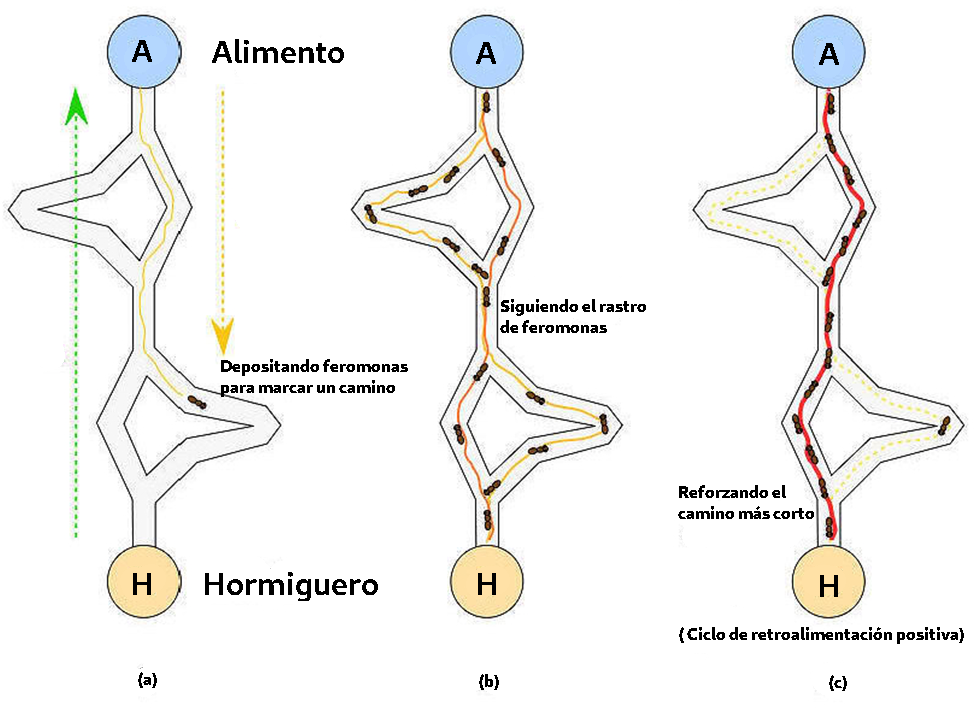
\includegraphics[scale=0.5]{imagenes/ACO-ant.png}
    \caption{Etapas de b\'usqueda de alimento y de comunicaci\'on entre hormigas. (a) Flecha verde refleja la direcci\'on de la  b\'usqueda aleatoria, mientras que la flecha amarilla indica como una hormiga va depositando feromonas. (b) Otras hormigas siguen rastros de feromonas existente, aportando con sus propias feromonas. (c) Convergencia de las hormigas sobre el camino m\'as corto en base a la cantidad de feromonas depositada por m\'ultiples hormigas mediante un ciclo de retroalimentaci\'on positiva. Fuente: \cite{liu2020improving}.}
    \label{fig:hormigas}
\end{figure}
%Imagen de un recorrido

El conjunto de caminos que recorren las hormigas, para ir del hormiguero hacia la fuente de alimento y de retorno, puede ser interpretado como un grafo que representa esta red de caminos. En esta representaci\'on, la b\'usqueda de caminos corresponde a encontrar conjuntos de nodos o aristas adyacentes, y una componente de soluci\'on $c_{i}$ corresponde a una arista, siendo el recorrido desde una arista inicial hasta una arista final. La construcci\'on de una soluci\'on utiliza hormigas artificiales, tambi\'en llamadas agentes, que se desplazan a trav\'es del grafo mediante aristas adyacentes. La elecci\'on de aristas en cada paso de la construcci\'on utiliza la informaci\'on de las feromonas de cada una de las aristas candidatas, formando la soluci\'on incrementalmente. La metaheur\'istica ACO, indicada en el Algoritmo \ref{ACO-Algo}, consiste en 4 etapas, donde las 3 \'ultimas no tienen un orden espec\'ifico.

\begin{algorithm}[H]
\SetAlgoLined
 Ajuste de Par\'ametros \& inicializaci\'on de feromonas\;
 \While{Criterio de finalización no se cumple}{
   Construcci\'on\_de\_soluci\'on\_de\_cada\_hormiga()\;
   M\'etodo\_de\_b\'usqueda\_no\_local(); //Paso opcional\\
   Actualizaci\'on\_de\_feromonas()\;
 }
 \caption{Algoritmo metaheur\'istica ACO}\label{ACO-Algo}
\end{algorithm}

%%% CAMI VA AQUI

\subsection{Adaptaci\'on de un modelo COP a una metaheur\'istica ACO}

Es posible adaptar la definici\'on del modelo COP al modelo de feromonas de la metaheur\'istica ACO, mediante la asociaci\'on entre la definici\'on de variable {\it instanciada} del modelo COP y lo que representa un componente de soluci\'on o arista en un recorrido de una hormiga. 
Espec\'ificamente, si se extiende la definici\'on de componente de soluci\'on $c_{i}$ para que esta pueda tener valores $v_{i}^{j}$ que var\'ien dependiendo de un dominio $D_i$, el componente de soluci\'on pasa a ser $c_{ij}$. As\'i se obtiene la equivalencia entre la asignaci\'on $X_i = v_{i}^{j}$ que representa una variable {\it instanciada} del modelo COP, y la selecci\'on de un componente de soluci\'on $c_{ij}$,  para una soluci\'on o camino $s$ en ACO\cite{socha2008ant}.
%equivalente a una arista en esta investigaci\'on,


Luego, la definici\'on de una soluci\'on $s$ puede representarse como un conjunto de componentes de soluci\'on $c_{ij} \in C, i = 1 \dotsc n, j = 1 \dotsc |D_i|$. A su vez, la feromona asociada a una componente de soluci\'on se transforma de $\tau_i$ a $\tau_{ij}$. El Algoritmo  \ref{ACO-Algo} se modifica acordemente para representar la equivalencia entre el modelo COP y la metaheur\'istica ACO, a\~nadiendose las definiciones de los datos y el resultado esperado, quedando como lo indica el algoritmo \ref{COP-ACO-Algo}. 


\begin{algorithm}[H]
\SetAlgoLined
\KwData{Variables $X_i \dotsc X_n$, dominios $D_1 \dotsc D_n$, Restricciones $\in \Omega$}
\KwResult{conjunto s\textquotesingle $ \subseteq S$ != $\emptyset$, si existen soluciones factibles}
 Ajuste de Par\'ametros \& inicializaci\'on de feromonas \;
 \While{Criterio de finalización no se cumple}{
   Construcci\'on\_de\_soluci\'on\_de\_cada\_hormiga()\;
   M\'etodo\_de\_b\'usqueda\_no\_local(); //Paso opcional\\
   Actualizaci\'on\_de\_feromonas()\;
 }
 \caption{Algoritmo de un modelo COP adaptado a una metaheur\'istica ACO}\label{COP-ACO-Algo}
\end{algorithm}

\section{Individualizaci\'on de filamentos mediante la metaheur\'istica ACO}
%similitud entre ambos
Se ha establecido en la secci\'on \ref{sec:OptiMethods} que una red de filamentos puede ser representada mediante un grafo, de forma similar a lo que sucede con la representaci\'on del conjunto de caminos que las hormigas recorren en b\'usqueda de alimento. En particular, un filamento en un grafo corresponde a un conjunto de aristas adyacentes, con lo que se puede asociar la individualizaci\'on de un filamento a la elecci\'on de una o m\'as aristas o componentes de soluci\'on, tal como se lleva a cabo en la metaheur\'istica ACO. A su vez, durante la elecci\'on de las aristas adyacentes que permiten individualizar un filamento, se puede utilizar una o m\'as caracter\'isticas que las aristas o componentes de soluci\'on poseen, para dirimir entre las aristas a elegir durante este proceso. Este comportamiento es similar al que las hormigas realizan utilizando las feromonas. Lo anterior constituye el fundamento para utilizar la metaheur\'istica ACO en el proceso de construcci\'on y evaluaci\'on de soluciones que permiten individualizar filamentos.

%Problema de explorar el espacio de soluciones
%comportamiento de las hormigas se puede asemejar a la forma en que los filamentos fueron creciendo o decreciendo.
La b\'usqueda de conjuntos de aristas adyacentes para individualizar uno o m\'as filamentos implica examinar un espacio de soluciones que no es posible de recorrer en tiempo polinomial, dado que sin restricciones las combinaciones crecen exponencialmente\cite{buchin2007number}\cite{biswas2012hamiltonian}. La metaheur\'istica ACO permite en sus distintas etapas (Construcci\'on de soluci\'on, b\'usqueda no local, actualizaci\'on de feromonas) incorporar informaci\'on que puede acotar el espacio de b\'usqueda. En el caso de la individualizaci\'on de filamentos, las diversas caracter\'isticas asociadas a las aristas, as\'i como las caracter\'isticas que definen el comportamiento global de un filamento permiten realizar esta tarea. 

\subsection{Inicializaci\'on de la metaheur\'istica ACO}

En el paso de inicializaci\'on de ACO se deben definir los valores de los par\'ametros relacionados a las heur\'isticas y de las feromonas utilizadas. Una de las caracter\'isticas m\'as relevantes para discriminar aristas en el proceso de construcci\'on corresponde al \'angulo que forman 2 aristas adyacentes.
El primer umbral que permite definir si ambas aristas pertenecen al mismo filamento se define como $\theta$. As\'i, si el \'angulo se encuentra en el rango $[0, \theta]$ se puede dirimir que ambas aristas pertenecen al mismo filamento. Un segundo umbral se define como $Max\_Angle$, que indica el l\'imite por sobre el cual se puede inferir que estas 2 aristas no pertenecen al mismo filamento. Estos par\'ametros dependen de la c\'elula observada, asignando a $\theta$ valores de 30\textdegree ~para microt\'ubulos de planta y de 45\textdegree~ para neuronas. $Max\_Angle$ depende de $\theta$ al definirse como el m\'aximo entre 2.5 veces $\theta$ y 90\textdegree.

Otros par\'ametros a utilizar corresponden a {\it Max\_Axial\_Displacement} y a {\it Max\_Score}. El primero hace referencia a la tolerancia al evaluar la diferencia entre la magnitud de 2 aristas adyacentes, y el \'angulo que conforman. Los valores de {\it Max\_Axial\_Displacement} son de 1.5 para el caso de los microt\'ublos de planta o de 2.5 para las neuronas. Por su parte, {\it Max\_Score} define el puntaje m\'aximo a obtener por un camino de buena calidad. Su valor durante este trabajo corresponde a 2, y es utilizado por la heur\'istica miope (ecuaci\'on \ref{eq:heuristicaMiope}), que se define m\'as adelante en la secci\'on \ref{subsubsec:antTourInit}. A su vez, los par\'ametros $\alpha$ y $\beta$ tambi\'en utilizados en la heur\'istica miope, que regulan la ponderaci\'on entre esta heur\'istica y las feromonas, son fijados en 1.


En el caso de las feromonas, se define un valor inicial de $\tau_{ij} = 1$, pero utilizando un concepto inverso de feromona con respecto al que se present\'o previamente. El cambio consiste en el uso de {\it anti-feromonas} o SAP ({\it Substractive Anti-Pheromone})\cite{montgomery2002anti}, que se explica en la secci\'on \ref{subsec:pheroUpdate} y consiste en disminuir el valor de la feromona asociada a su respectiva arista. El uso de SAP introduce el par\'ametro $\gamma$, el que se define en 0.5 en base a lo encontrado en la literatura.

%%%%%%%%%%%%%%%%%%%%%%%%%%%%%%%%%%%%%%%%
%Para las feromonas se configura el valor inicial de $\tau_{ij}$ en 1 para los pares $\langle c_{ij}$,$ seg_{n}\rangle \> \forall c_{ij} \in \> ]\theta, Max\_Angle]$, dado que al usar SAP esta probabilidad se ir\'a reduciendo de acuerdo a un factor $\gamma$ seg\'un lo explicado en la secci\'on \ref{subsec:pheroUpdate}. El valor de $\gamma$ se define en 0.5, en base a lo encontrado en la literatura.
%%%%%%%%%%%%%%%%%%%%%%%%%%%%%%%%%%%%%

Finalmente, el criterio de finalizaci\'on consiste en generar nuevas hormigas artificiales hasta que todas las aristas sean parte de al menos una soluci\'on de buena calidad, o que el n\'umero de hormigas generadas sea superior a 4 veces la cantidad de aristas. En lo que sigue de este trabajo se utiliza el t\'ermino hormigas en referencia a las hormigas artificiales o agentes.


\subsection{M\'etodo de construccion de soluci\'on de cada hormiga}
\label{subsubsec:antTourInit}
Al comenzar un recorrido, cada hormiga es asignada una arista de acuerdo a la heur\'istica de asignaci\'on inicial, la que corresponde al primer elemento del camino o recorrido parcial $s^{P}$. La heur\'istica de asignaci\'on inicial analiza hasta 3 situaciones, dependiendo del tipo de c\'elula:
\begin{enumerate}
\item La arista a asignar debe tener al menos uno de sus nodos con grado 1, indicando que es el inicio o final de una parte del grafo.

\item De no haber aristas disponibles con esas caracter\'isticas, se realiza una asignaci\'on inicial de una arista que cumpla con 2 criterios:
\begin{itemize}
    \item Tener uno de sus nodos con grado 2 o superior.
    \item El \'angulo que forma la arista candidata a elegir, junto a otra arista a la que pertenece el nodo, debe pertenecer al rango $]\theta, Max\_Angle]$.
\end{itemize}
%$\theta$ es un umbral que define el \'angulo m\'aximo, en grados, bajo el que se considera que 2 aristas contiguas respetan la rectitud necesaria para formar parte del mismo filamento. $Max\_Angle$ es un umbral que define el \'angulo m\'aximo, en grados, por sobre el cual se descarta de forma absoluta que 2 aristas contiguas forman parte del mismo filamentos. Este rango delimita los pares de aristas que a priori no representan combinaciones que respetan el criterio de rectitud, pero cuya explicaci\'on puede encontrarse en variaciones inducidas durante la extracci\'on del grafo desde la imagen, por lo que es necesario incorporar la exploraci\'on de estos pares de aristas.

\item De no existir aristas con alg\'un nodo que cumpla con los dos criterios previos, es posible asignar una arista aleatoria. Esta arista no debe pertenecer al una soluci\'on o camino evaluado como de buena calidad. La calidad de un camino se presenta m\'as adelante en esta secci\'on.
\end{enumerate}

%a elecci\'on de un componente $c_{ij}$ por una hormiga durante la construcci\'on de un camino, se lleva a cabo mediante el c\'alculo de una probabilidad para cada componente $c_{ij}$ posible de elegir. Este conjunto de vecinos factibles se denomina $N(s^{P}) \subseteq C$. En la probabilidad de selecci\'on influye el camino ya escogido, denominado soluci\'on parcial $s^{P}$. 

% a diferencia de otros ACO, aca s^P != \emptyset al comienzo
Una vez asignada la primera arista seg\'un la heur\'istica previamente descrita, cada hormiga debe avanzar mediante la elecci\'on de nuevas aristas para a\~nadirlas a su recorrido. Este procedimiento corresponde a la probabilidad de elegir una arista o componente $c_{ij}$ a partir de un conjunto de aristas vecinas $N(s^{P})$. Las aristas que pertenecen a $N(s^{P})$ son s\'olo las aristas adyacentes a la \'ultima arista agregada a la soluci\'on parcial $s^P$ que son factibles de agregar a la soluci\'on parcial. La factibilidad de a\~nadir una arista de $N(s^{P})$ a $s^{P}$ corresponde a la probabilidad expresada en la ecuaci\'on \eqref{eq:antProbabilities}. Esta probabilidad depende del valor de la feromona $\tau_{ij}$ asociada a la arista $c_{ij}$, as\'i como del valor de la heur\'istica miope $\eta_{ij}$ (ecuaci\'on \ref{eq:heuristicaMiope}) que eval\'ua el \'angulo formando entre la arista $c_{ij} \in N(s^{P})$ y la \'ultima arista agregada a $s^{P}$, que se define como $s_{n}^{P}$.


En particular, la heur\'istica miope $\eta_{ij}$ entrega una puntuaci\'on que disminuye a medida que el \'angulo mencionado aumenta, siendo el rango $[0, \theta]$ el que otorga la puntuaci\'on m\'axima de $Max\_Score$. Si el \'angulo es mayor a $Max\_Angle$ la puntuaci\'on corresponde a 0. Para el rango intermedio $]\theta, Max\_Angle]$, la puntuaci\'on depende de la diferencia entre el \'angulo formando entre la arista $c_{ij} \in N(s^{P})$ y $s_{n}^{P}$. Mientras m\'as aumenta esta diferencia, menor es la puntuaci\'on asignada.


%que tiene asociada. Otro aspecto que influye en la elecci\'on de una arista es la desviaci\'on que puede ocasionar si se a\~nade a $s^P$, con respecto a la rectitud del camino ya recorrido. Esta evaluaci\'on se refleja en el valor $\eta_{ij}$ asociado a la arista, que se calcula mediante la heur\'istica miope. 
%mediante la heur\'istica miope (ecuaci\'on \eqref{eq:heuristicaMiope}) que privilegia los candidatos que causen la menor desviaci\'on en la rectitud del camino. 
%Se define que las aristas $c_{ij}$ que aportan con mayor probabilidad a la menor desviaci\'on son aquellos que en conjunto con el \'ultimo elemento elegido por la hormiga en ese punto ($c_{(i-1)j}$) forman un \'angulo en el rango $[0, \theta]$. El criterio de finalizaci\'on para la hormiga corresponde a que el conjunto $N(s^{P}) = \emptyset$, es decir, que no existan opciones de aristas para seleccionar.

%P(C_{ij} | s^{P}) = P_{n_{i},n_{j}} = P_{e_{x}}
\begin{equation}
P(c_{ij} | s^{P}) = \frac
        {\tau_{ij}^{\alpha} \times \eta_{ij}^{\beta}}
        {\sum\limits_{c_{ij}\in N(s^p)}{\tau_{ij}^{\alpha} \cdot \eta_{ij}^{\beta} } }, \forall c_{ij} \in N(s^{P}).
\label{eq:antProbabilities}
\end{equation}

La evaluaci\'on de \'angulos entre aristas adyacentes que pertenezcan al rango intermedio $]\theta, Max\_Angle]$ en la heur\'istica miope, facilita la exploraci\'on de soluciones o caminos que de forma miope no califican como soluciones candidatas factibles de representar un filamento, pero que tampoco pueden ser descartados completamente. En el caso que un camino tenga uno o m\'as pares de aristas adyacentes cuyo \'angulo pertenezca a este rango, se definir\'a el camino como de {\it calidad intermedia}.

%Otro aspecto de la ecuaci\'on \eqref{eq:heuristicaMiope} radica en la posibilidad de elecci\'on de aristas $c_{ij}$ que tienen un \'angulo en el rango $]\theta, \text{Max\_Angle}]$ con el componente de soluci\'on $c_{(i-1)j}$. Esto facilita la exploraci\'on de soluciones/caminos que de forma miope aparecen como de calidad no \'optima, y que para los efectos de este trabajo se denominan como de {\it calidad intermedia}. Esta evaluaci\'on consistente en disminuir la probabilidad de elecci\'on a medida que se incrementa la diferencia entre el \'angulo que forman $c_{ij}$ y $c_{(i-1)j}$, y la mitad de $\theta$.
%donde cada uno representa a una arista en esta investigaci\'on, y . Al momento de que la diferencia sea 90\textdegree, la probabilidad de asignaci\'on se reduce al 50\% de la probabilidad de un componente $c_{ij} \in [0, \theta]$.

\begin{equation}
    \eta_{ij} = 
        \begin{cases} 
        \text{Max\_Score si } \measuredangle(c_{ij}, s_{n}^{P}) \in [0, \theta]\\[3ex],
        
        \text{Max\_Score} \cdot \left(1 - \dfrac{ \left| \measuredangle(c_{ij}, s_{n}^{P}) - \frac{\theta}{2} \right|} {180} \right)  \text{ si } \measuredangle(c_{ij}, s_{n}^{P}) \in \quad ]\theta, \text{Max\_Angle}],\\[3ex]
        
        \text{0 en otro caso.}
        \end{cases}
    \label{eq:heuristicaMiope}
\end{equation}

Con la finalidad de cuantificar la calidad de la soluci\'on construida por una hormiga, en cada selecci\'on de arista realizada, se suma el resultado de la heur\'istica miope $\eta_{ij}$ a la calidad del camino que la hormiga lleva hasta ese punto. Cada hormiga comienza con una calidad 0, que al finalizar su recorrido es dividida por el n\'umero de aristas menos 1, para normalizar el valor entre las distintas soluciones. Se establece que para ser consideradas como una soluci\'on de {\it buena calidad}, la hormiga debe tener una calidad mayor o igual a $Max\_Score/2$. Es importante destacar que la calidad de una soluci\'on puede variar en cada etapa de la metaheur\'istica ACO, pudiendo descartarse una soluci\'on en base a los criterios de cada m\'etodo. El desechar una soluci\'on implica ajustar su calidad a 0, lo que la clasifica como de {\it mala calidad}. Las hormigas que en cada elecci\'on de arista hayan elegido componentes $c_{ij}$ que formaban un \'angulo en en rango $[0, \theta]$ con $s_{n}^{P}$, son las que obtienen el m\'aximo puntaje de $Max\_Score$ al normalizarse, y se definen como de {\it calidad \'optima}. Los caminos clasificados como de {\it calidad intermedia} son inicialmente parte del grupo de soluciones de buena calidad.

%Un planteamiento similar a lo anterior es el {\it Path Cover Problem} o PCP, en el que se descompone un grafo dirigido en caminos con el objetivo de obtener un conjunto de caminos. Cada nodo o arista debe pertenecer exactamente a un camino y los caminos pueden comenzar o terminar en cualquier parte del grafo.

%Esta reducci\'on del espacio de b\'usqueda debe considerar no eliminar soluciones o caminos v\'alidos, como puede suceder con casos de cruce o solapamiento de filamentos, o la existencia de ciclos. 


%En el caso de la individualizaci\'on de filamentos, es necesario que la definici\'on del problema considere como v\'alidos caminos que representen los casos de filamentos con o sin ciclos, as\'i como superposici\'on y/o cruce. Lo anterior impide forzar la pertenencia de un nodo o arista a un s\'olo camino


\subsection{M\'etodo de actualizaci\'on de feromonas}
\label{subsec:pheroUpdate}
Una vez que la hormiga termina un recorrido, se eval\'ua su calidad para actualizar las feromonas $\tau_{ij}$ asociadas a los componentes de soluci\'on que lo conforman. As\'i, en una metaheur\'istica ACO tradicional, se aumenta el valor de $\tau_{ij}$ en cada $c_{ij}$ que es parte de un camino de buena calidad. Adicionalmente, los valores de las feromonas sufren decaimiento en el tiempo, dado por el par\'ametro $\rho$, que busca evitar la convergencia que las feromonas pueden causar en caminos de buena calidad obtenidos al inicio de las iteraciones.


En la individualizaci\'on de filamentos, se utilizan {\it anti-feromonas}, con el prop\'osito de indicar a las hormigas de futuras iteraciones los caminos que no son de buena calidad. La diferencia radica en que las anti-feromonas buscan acotar el espacio de soluciones $S$ sin necesariamente buscar la convergencia sobre un \'unico camino. Este cambio implica no utilizar el par\'ametro $\rho$, ya que no existe decaimiento en este uso de anti-feromonas, y reemplazarlo por el par\'ametro $\gamma$ como factor de reducci\'on/penalizaci\'on\cite{montgomery2002anti}. Al ser la penalizaci\'on un factor que se aplica sobre el valor de $\tau_{ij}$, la anti-feromona puede disminuir constantemente sin llegar a valer exactamente cero, por lo que se define un l\'imite de 2 penalizaciones como m\'aximo para cada anti-feromona. Al alcanzar este l\'imite, se reduce el valor de $\tau_{ij}$ a 0, haciendo imposible la elecci\'on de la arista $c_{ij}$ respectiva.
%para las hormigas cuya soluci\'on parcial $s^{P}$ contenga el segmento en el par $<$componente,segmento$>$ penalizado. 

Adem\'as de cambiar el uso de feromonas por el de anti-feromonas, se introduce una segunda modificaci\'on, relativa a las aristas a las que aplica la penalizaci\'on de las anti-feromonas. Un uso tradicional de anti-feromonas implica la disminuci\'on del valor de $\tau_{ij}$ para su respectiva arista $c_{ij}$, en caso de que se trate de un camino de mala calidad. 
Esto puede llevar a la p\'erdida de exploraci\'on de soluciones en la individualzaci\'on de filamentos, ya que una arista con un $\tau_{ij}$ penalizado por pertenecer a uno o m\'as caminos de mala calidad, puede bloquear otros caminos, dado que el valor de $\tau_{ij}$ no guarda relaci\'on con el conjunto de aristas que causa la penalizaci\'on. As\'i, las soluciones que pudiesen pasar por esa arista se ven limitadas.

 
%En aquel caso, la \'unica arista de $seg_{n+1}$ se transforma en un cuello de botella para la exploraci\'on debido a que penaliza de forma indiscriminada a todas las hormigas que pasen por ah\'i, independientemente del \'angulo que forme con otras aristas o componentes. Para subsanar aquel caso, a este tipo de segmentos se le a\~naden los nodos del segmento que lo precede, $seg_{n}$, con el objetivo de evitar que el an\'alisis del par $seg_{n+1}$ con la componente $c_{ij}$ que inicia el segmento $n+2$ sea s\'olo de 2 aristas.

En este trabajo se propone que la penalizaci\'on de $\tau_{ij}$ guarde relaci\'on con el conjunto de aristas en el camino $s$ que preceden a la arista $c_{ij}$. Se define a aquel conjunto de aristas como un segmento de un camino recorrido por la hormiga $a$, expresado como $seg_{n}^{a}$. Los segmentos se generan durante la construcci\'on de un recorrido, existiendo siempre al menos un segmento en cada camino. Dado que el \'angulo entre 2 aristas adyacentes es uno de los criterios utilizados durante la construcci\'on de un camino, el fin de un segmento puede suceder en 2 casos: si la \'ultima arista en el camino corresponde al final del recorrido, o si la arista $s_{n}^{P}$ (la \'ultima arista agregada a $s^P$) forma un \'angulo en el rango $]\theta, Max\_Angle]$ con la arista $c_{ij} \in N(s^P)$ a agregar a la soluci\'on parcial.

\begin{figure}[h!]
    \centering
    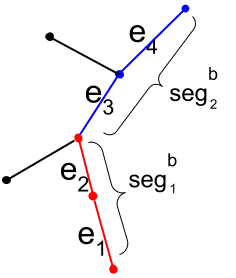
\includegraphics{imagenes/ant_segments_simple_case.png}
    \caption{Camino de una hormiga $b$ compuesto por 2 segmentos. El \'angulo entre las aristas $e_2$ y $e_3$ pertenece al rango $]\theta, Max\_Angle]$, finalizando el segmento $seg^{b}_1$ e iniciando el segmento $seg^{b}_2$. Fuente: Elaboraci\'on Propia.}
    \label{fig:segmentSimpleCase}
\end{figure}

As\'i, cada segmento esta formado por una o m\'as aristas, donde cada arista del segmento forma un \'angulo en el rango $[0, \theta]$ con sus vecinos. Un ejemplo de esto se puede observar en la Figura \ref{fig:segmentSimpleCase}, en el que si se penaliza la arista $e_3$, esta penalizaci\'on ser\'a asociada al segmento $seg^{b}_{1}$, disminuyendo la posibilidad de que futuras hormigas que recorran este segmento escojan $e_3$, sin perjuicio de otros caminos que pasen por $e_3$ pero no por el segmento $seg^{b}_{1}$.


Una ventaja de utilizar segmentos de camino es evitar volver a evaluar la relaci\'on entre todas las aristas que conforman el camino, ya que las aristas que conforman un segmento cumplen con un criterio para ser consideradas como parte del mismo filamento. As\'i, la evaluaci\'on de la calidad del camino se realiza s\'olo en el caso que 2 aristas vecinas formen un \'angulo de rango intermedio ($]\theta, Max\_Angle]$), enfoc\'andose en las soluciones de calidad intermedia que permiten explorar el espacio de soluciones.


Se debe se\~nalar que esta propuesta de penalizaci\'on realiza la evaluaci\'on de la calidad del camino en orden inverso al utilizado durante la construcci\'on del recorrido, imitando el retorno que realiza una hormiga desde el alimento hacia su hormiguero. Esto, sumando al uso de segmentos, permite comenzar la revisi\'on en el \'ultimo par de aristas cuyo \'angulo pertenece al rango intermedio, es decir, el nodo donde termina el pen\'ultimo segmento y comienza el \'ultimo. A modo de ejemplo, en la Figura \ref{fig:segmentSimpleCase}, esto ser\'ia el nodo com\'un de las aristas $e_2$ y $e_3$, que separa los segmentos $seg^{b}_1$ y $seg^{b}_2$. En este ejemplo, en caso de penalizar la arista $e_3$, ser\'a solo disminuyendo su posibilidad de ser elegida para caminos que contengan al segmento $seg^{b}_1$ en su soluci\'on.

%cortar de atras para adelante una sola vez permite acotar los caminos malos sin descartar una solucion completamente, solo sacando la parte potencialmente mala al final


Por \'ultimo en este aspecto, y a diferencia del uso tradicional de feromonas o anti-feromonas, donde se penalizan todas las aristas pertenecientes a una soluci\'on, el recorrido inverso y el uso de segmentos permite que sea suficiente la penalizaci\'on de una arista en la soluci\'on para clasificar la soluci\'on $s$ como de mala calidad y desecharla. Esto permite que a partir de una soluci\'on de mala calidad se remueva el \'ultimo segmento, permitiendo a otra hormiga recorrer un camino similar con un distinto final, favoreciendo la exploraci\'on. Para visualizar esto, es posible utilizar la Figura \ref{fig:segmentComplexCaseH}, en donde una hormiga pudiese construir un camino incorporando las aristas $e_1$, $e_2$, $e_4$, $e_5$ y $e_6$. Al desechar el \'ultimo segmento, conformado s\'olo por la arista $e_6$, permite que otra hormiga recorra desde $e_1$ hasta $e_5$, pudiendo agregar $e_7$ a su camino o terminando en $e_5$. 

\begin{figure}[h!]
    \centering
    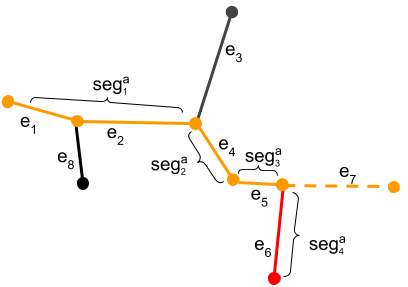
\includegraphics{imagenes/ant_segments_complex_case_H.png}
    \caption{Camino de una hormiga $a$ compuesto por 4 segmentos. El comienzo en orden inverso a la construcci\'on favorece la exploraci\'on, reemplazando el \'ultimo segmento por otro o simplemente concluyendo el recorrido. Fuente: Elaboraci\'on Propia.}
    \label{fig:segmentComplexCaseH}
\end{figure}

%Existen $N + 1$ segmentos en $s$ si la soluci\'on contiene $N$ elementos $c_{ij} \in ]\theta, 90]$ (de calidad intermedia). 
Lo anterior permite definir que la penalizaci\'on de $\tau_{ij}$ este asociada a la arista $c_{ij}$ y al segmento que precede a $c_{ij}$ en el recorrido de una hormiga $a$. El segmento que precede a $c_{ij}$ en un camino $s$ se define como $seg^{a}_{prev}$. Adicionalmente, se tiene que entre distintos caminos pueden existir segmentos equivalentes, lo que sucede en el caso de que contengan las mismas aristas. Esto permite que se refieran al mismo valor $\tau_{ij}$ a pesar de los nombres relativos al camino al que pertenecen. 

 \begin{figure*}[h]
    \centering
    \begin{subfigure}[t]{0.48\textwidth}
        \centering
        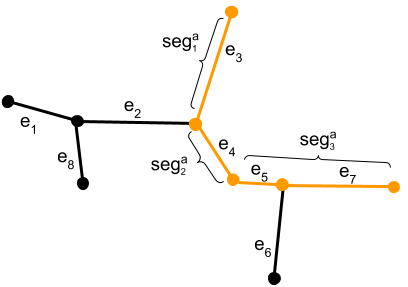
\includegraphics[height=2in]{imagenes/ant_segments_complex_case_1.png}
        \caption{Camino de una hormiga $a$ que contiene las aristas $e_3$, $e_4$, $e_5$ y $e_7$.}
        \label{fig:segmentComplexCase1}
    \end{subfigure}%
    ~ \hspace{0.5cm}
    \begin{subfigure}[t]{0.48\textwidth}
        \centering
        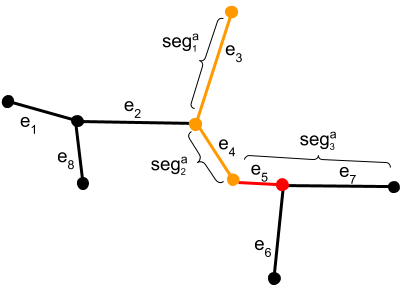
\includegraphics[height=2in]{imagenes/ant_segments_complex_case_2.png}
        \caption{Penalizaci\'on del camino de la hormiga $a$ en la arista $e_5$ con respecto al segmento $seg^{a}_2$ conformado solo por la arista $e_4$.}
        \label{fig:segmentComplexCase2}
    \end{subfigure}

\vskip\baselineskip
    \begin{subfigure}[t]{0.48\textwidth}
        \centering
        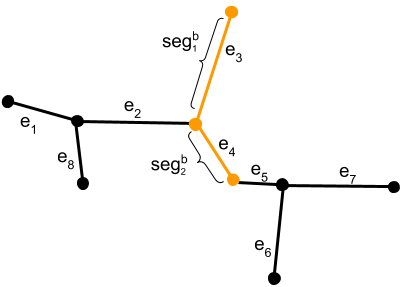
\includegraphics[height=2in]{imagenes/ant_segments_complex_case_4.png}
	    \caption{Camino de una hormiga $b$ que contiene las aristas $e_3$, $e_4$. El camino $b$ no puede agregar la arista $e_5$ debido a que se encuentra penalizada para el segmento formado por la arista $e_4$.}
        \label{fig:segmentComplexCase3}
    \end{subfigure}%
    ~ \hspace{0.5cm}
    \begin{subfigure}[t]{0.48\textwidth}
        \centering
        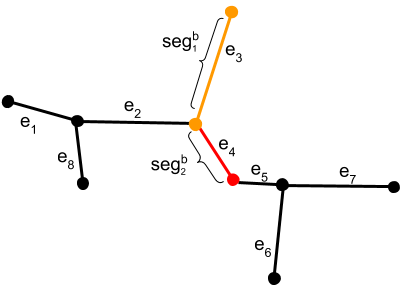
\includegraphics[height=2in]{imagenes/ant_segments_complex_case_5.png}
        \caption{Penalizaci\'on del camino de la hormiga $b$ en la arista $e_4$ con respecto al segmento $seg^{b}_1$ conformado solo por la arista $e_3$.}
        \label{fig:segmentComplexCase4}
    \end{subfigure}

    \vskip\baselineskip

    \begin{subfigure}[t]{\textwidth}
        \centering
        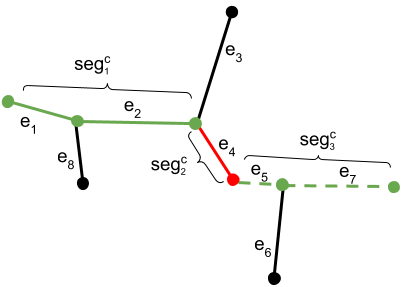
\includegraphics[height=2in]{imagenes/ant_segments_complex_case_block.png}
	    \caption{El camino de la hormiga $c$ no puede pasar de la arista $e_4$ en el caso que la penalizaci\'on no tenga relaci\'on con el segmento que precede a esa arista.}
        \label{fig:segmentComplexCaseBlocked}
    \end{subfigure}
    \caption{Funcionamiento de la propuesta de penalizaci\'on de anti-feromonas con segmentos y recorrido inverso. Por simplicidad se supone que la penalizaci\'on de $\tau_{ij}$ solo una vez es suficiente para eliminar la posibilidad de elegir una arista $c_{ij}$. En este ejemplo, los caminos $a$ y $b$ se desechan por evaluarse como de mala calidad. El camino es penalizando en $e_4$ respecto al segmento que lo precede. El camino $c$ puede seleccionar la arista $e_4$ ya que esta arista no se encuentra penalizada con respecto al segmento $seg^{c}_1$, pudiendo luego agregar el segmento $seg^{c}_3$.Fuente: Elaboraci\'on Propia.}
    \label{fig:segmentComplexCase}
\end{figure*}

Un caso particular en el que esta propuesta puede sufrir del mismo problema de cuello de botella que intenta evitar, es al momento que un segmento formado por s\'olo una arista se encuentre entre 2 segmentos. Este situaci\'on, reflejada en la Figura \ref{fig:segmentComplexCase}, implica que la penalizaci\'on efectuada a los caminos de las hormigas $a$ y $b$ pueden generar un bloqueo del camino de la hormiga $c$, dado que tras la penalizaci\'on efectuada en la evaluaci\'on de $b$, se tiene un segmento conformado solo por la arista $e_4$, la que forma un \'angulo que pertenece al rango $]\theta, Max\_Angle]$ con cada uno de sus vecinos.

%Si el camino continua siendo de .... otras hormigas pueden intentar iterativamente 
%explicar q la penalizacion es solo necesaria en soluciones de calidad intermedia

Para subsanar aquel caso, a los segmentos de s\'olo una arista, se le a\~naden las aristas del segmento que lo precede con el objetivo de evitar que el an\'alisis sea s\'olo entre 2 aristas. As\'i, en 

del par $seg_{n+1}$ con la arista $c_{ij}$ ($e_4$ e

 \begin{figure*}[h]
    \centering
    \begin{subfigure}[t]{0.48\textwidth}
        \centering
        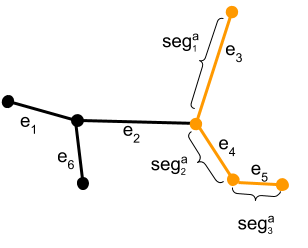
\includegraphics[height=2in]{imagenes/ant_segments_complex_case_B1.png}
        \caption{Camino de una hormiga $a$ que contiene las aristas $e_3$, $e_4$ y $e_5$.}
        \label{fig:segmentComplexCaseB1}
    \end{subfigure}%
    ~ \hspace{0.5cm}
    \begin{subfigure}[t]{0.48\textwidth}
        \centering
        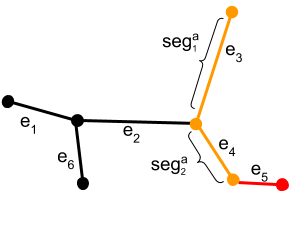
\includegraphics[height=2in]{imagenes/ant_segments_complex_case_B2.png}
        \caption{Penalizaci\'on del camino de la hormiga $a$ en la arista $e_5$ con respecto al segmento $seg^{a}_2$ conformado solo por la arista $e_4$.}
        \label{fig:segmentComplexCaseB2}
    \end{subfigure}

\vskip\baselineskip
    \begin{subfigure}[t]{0.48\textwidth}
        \centering
        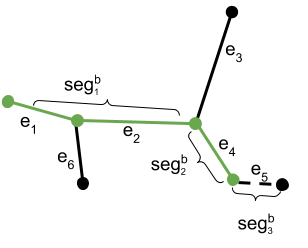
\includegraphics[height=2in]{imagenes/ant_segments_complex_case_B_blocked.png}
	    \caption{Camino de una hormiga $b$ que contiene las aristas $e_1$, $e_2,$ y $e_4$. El camino $b$ no puede agregar la arista $e_5$ debido a que se encuentra penalizada para el segmento conformado por la arista $e_4$, que corresponde al $seg^{a}_2$.}
        \label{fig:segmentComplexCaseBBlocked}
    \end{subfigure}%
    ~ \hspace{0.5cm}
    \begin{subfigure}[t]{0.48\textwidth}
        \centering
        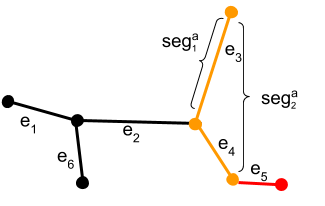
\includegraphics[height=2in]{imagenes/ant_segments_complex_case_B2_extended.png}
        \caption{Soluci\'on propuesta para los segmentos de solo 1 arista no causen bloqueos como el que afecta a la hormiga $b$, mediante la extensi\'on del segmento, a\~nadiendo el segmento anterior.}
        \label{fig:segmentComplexCaseB2Extended}
    \end{subfigure}

    \caption{Caminos de las hormigas $a$ y $b$. Para evitar que la penalizaci\'on sobre $e_5$ por el segmento que lo precede, $seg^{a}_2$, bloquee el camino $b$, se modifica el inicio del segmento asociado a la penalizaci\'on, incorporando las aristas del segmento previo, $seg^{a}_2$. As\'i se mantiene la l\'ogica de asociar la penalizaci\'on no solo a la arista sino que tambi\'en al segmento que la precede. Estos casos suceden para aristas como $e_4$, que forman \'angulos en el rango $]\theta, Max\_Angle]$ con todas sus aristas vecinas, quedando solas en un segmento de largo 1. Fuente: Elaboraci\'on Propia.}
    \label{fig:segmentComplexCaseB}
\end{figure*}


%La perdida de exploraci\'on tambi\'en sucede en el caso que el segmento $seg_{n+1}$ contenga solo 1 arista y no sea el segmento en el que finaliza el recorrido de la hormiga. En aquel caso, la \'unica arista de $seg_{n+1}$ se transforma en un cuello de botella para la exploraci\'on debido a que penaliza de forma indiscriminada a todas las hormigas que pasen por ah\'i, independientemente del \'angulo que forme con otras aristas o componentes. 

%Luego, mediante la anti-feromona se relaciona un segmento $seg^{a}_n \subset s$ y la componente de soluci\'on $c_{ij} \in seg_{n+1} \in s$, donde la elecci\'on de la arista o componente $c_{ij}$ despu\'es de haber elegido las aristas pertenecientes a $seg_n$ origina una soluci\'on de mala calidad. 

\subsection{Criterios para la actualizaci\'on de feromonas}

La anti-feromona se aplica sobre hormigas que han finalizado su recorrido, cuya calidad normalizada se encuentre entre $[Max\_Score/2, Max\_Score[$. Aquello implica que al menos un par de las aristas del recorrido forma un \'angulo que pertenece al rango intermedia $]\theta, Max\_Angle]$, necesitando un an\'alisis adicional para determinar si corresponde a una soluci\'on de buena calidad. 

......

El an\'alisis adicional se separa en evaluaciones comunes que no dependen de la c\'elula observada, agregando posteriormente las evaluaciones particulares. El conjunto de evaluaciones comunes consisten en evaluar la curvatura del recorrido, como tambi\'en la magnitud del desplazamiento entre la proyecci\'on de un segmento en relaci\'on a otro segmento contiguo. La evaluaci\'on particular se acciona si la c\'elula es una neurona, debido a que se requiere verificar que la finalizaci\'on del recorrido no sea en una arista que cumpla con el primer criterio de la heur\'istica de asignaci\'on de aristas iniciales, descrita en la secci\'on \ref{subsubsec:antTourInit}.

La curvatura de recorrido de una hormiga $a$ es el \'angulo formado por el nodo inicial ($n_{a1}$), el centro de masa de la misma hormiga ($mc_{a}$) y el nodo final ($n_{af}$). Este \'angulo no debe superar el umbral definido al multiplicar el \'angulo $\theta$ por un factor denominado {\it Max\_Axial\_Displacement}. Este factor permite flexibilizar la tolerancia de la curvatura en base a $\theta$. Si el recorrido de la hormiga tiene un \'angulo igual o mayor al umbral, implica que la soluci\'on encontrada es demasiado curva para representar un filamento, por lo que se penaliza el par $\langle c_{ij}$,$ seg_{n}\rangle$ donde $c_{ij}$ es la componente de soluci\'on/arista que inicia el \'ultimo segmento de la hormiga, mientras que $seg_{n}$ es el segmento que lo precede. Posterior a la penalizaci\'on, se desecha la soluci\'on. El criterio de curvatura se refleja en la ecuaci\'on \eqref{eq:antiPheroSAP_Angle}.
%\begin{equation}
%    \label{eq:antiPheroSAP_Angle}
%    \tau_{ij} \leftarrow \tau_{ij} \cdot \gamma \quad \forall \langle c_{ij},seg_{n}\rangle > \textrm{Max\_Axial\_Displacement}
%\end{equation}

\begin{equation}
    \tau_{ij} \leftarrow
        \begin{cases}
        \tau_{ij} \cdot \gamma \text{ si } \measuredangle((n_{a1}, mc_{a}), (mc_{a}, n_{af})) < \theta \cdot \text{Max\_Axial\_Displacement},\\[3ex]
        
        \text{0 si } \tau_{ij} \leq 0.25, \\[3ex]
        \tau_{ij} \quad \text{en otro caso.}
        \end{cases}
    \label{eq:antiPheroSAP_Angle}
\end{equation}

%agregar referencia? tindemans rod straightness \cite{hawkins2010model} of MTs o 
El an\'alisis respecto a la magnitud del desplazamiento entre la proyecci\'on de un segmento en relaci\'on a los segmentos que lo preceden se fundamenta en la rigidez que algunos tipos de filamentos como los microt\'ubulos y los filamentos de actina poseen\cite{stam2017filament}. El criterio de rigidez consiste en analizar los segmentos con respecto a la totalidad de sus predecesores, comenzando por el \'ultimo segmento recorrido por la hormiga, es decir, desde el extremo final de la soluci\'on. A partir de cada par de $<$segmento,segmentos$_$predecesores$>$, $\langle seg_{n}$,$seg_{1,n-1}\rangle$, se debe seleccionar el miembro del par de mayor longitud, definido como $s_{max} = \max(\norm{seg_{n}}, \norm{seg_{1,n-1}})$, para calcular el \'angulo suplementario que forma con respecto al otro miembro del par, definido como $s_{min}$. El \'angulo suplementario, $\measuredangle supl(s_{max},s_{min})$ es el equivalente a calcular el \'angulo entre la proyecci\'on de $s_{max}$ y $s_{min}$.

Luego $s_{min}$ es multiplicado por el seno del \'angulo suplementario, estableciendo el desplazamiento con respecto al eje que forma $s_{max}$ y su proyecci\'on. El umbral que delimita al desplazamiento calculado previamente se define como el m\'ultiplo de $s_{max}$ por 10\% de {\it Max\_Axial\_Displacement}. 

Si el \'angulo suplementario es menor a $\theta$, se puede declarar que se cumple el criterio de rigidez. Lo anterior se refleja en la ecuaci\'on \eqref{eq:antiPheroSAP_Axial}. 


%Esta propiedad puede ser utilizada para delimitar como un segmentos de una hormiga se relacionan con el resto de la soluci\'on, ya que estos ser\'ia un reflejo indirecto de los movimientos din\'amicos de un filamento en el tiempo, capturados en un punto a trav\'es de una imagen. 
%La rigidez de un filamento puede describirse mediante la relaci\'on que existe entre un segmento de una hormiga, con respecto a todos los segmentos que lo preceden. 
\begin{equation}
    \tau_{ij} \leftarrow
        \begin{cases}
        \begin{split}
         \tau_{ij} \cdot \gamma \text{ si } & \sin(\measuredangle supl(s_{max},s_{min}) > s_{min} \cdot 0.1 \cdot \text{Max\_Axial\_Displacement} \\ & \land \measuredangle supl(s_{max},s_{min}) > \theta    
        \end{split}
        \\[3ex]
        
        \text{0 si } \tau_{ij} \leq 0.25 \\[3ex]
        \tau_{ij} \quad \text{en otro caso}
        \end{cases}
    \label{eq:antiPheroSAP_Axial}
\end{equation}

Si ambas evaluaciones son completadas correctamente y no existen evaluaciones particulares para la c\'elula observada, se declara a la soluci\'on como de buena calidad para un camino que representa un filamento. A diferencia de los filamentos de otras c\'elulas incluidas en este trabajo, el comportamiento esperado de los filamentos en una neurona permite caracterizar los lugares desde los cuales nuevos filamentos pueden generarse. Esta informaci\'on adicional se incorpora mediante la evaluaci\'on particular de un recorrido en una neurona, buscando validar el comportamiento esperado de un filamento, en relaci\'on a que los filamentos de una neurona parten del {\tt soma} o centro de la misma, y que filamentos posteriores que no comiencen del soma s\'olo pueden nacer a partir de otros filamentos. Un camino que termine en un nodo final de grado de 1 no respeta aquel comportamiento, debido a que en un grafo que representa una red de filamentos de una neurona, los nodos ubicados en el soma o en la intersecci\'on entre filamentos presentan un grado mayor a 1. La penalizaci\'on mediante la anti-feromona para este caso particular se refleja en la ecuaci\'on \ref{eq:antiPheroSAP_neuron}.

\begin{equation}
    \tau_{ij} \leftarrow
        \begin{cases}
         \tau_{ij} \cdot \gamma \text{ si } deg(n_{af}) = 1  \\[3ex]
        
        \text{0 si } \tau_{ij} \leq 0.25 \\[3ex]
        \tau_{ij} \quad \text{en otro caso}
        \end{cases}
    \label{eq:antiPheroSAP_neuron}
\end{equation}

%Finalmente, la ecuaci\'on \eqref{eq:antiPheroSAP} refleja la aplicaci\'on de las {\it anti-feromonas} sobre el par $\langle c_{ij}$,$ seg_{n}\rangle \forall c_{ij} \in ]\theta, Max\_Angle]$  donde $c_{ij} \in seg_{n+1}$, y cuya elecci\'on dio lugar a $seg_{n+1}$ que se aleja del desplazamiento axial m\'aximo que un filamento puede soportar.

En relaci\'on a los dominios $D_i$ declarados en la definici\'on del modelo de un COP, se destaca que en el caso de la individualizaci\'on de filamentos existe solo $D_1 \in D$, ya que la instanciaci\'on de variables ($X_i = v_{i}^{j}$ o $c_{ij}$) tiene una sola asignaci\'on posible, lo que lleva a una simplificaci\'on del componente $j$ en las ecuaciones presentadas.

\subsection{M\'etodo de b\'usqueda no local}
Una vez que la hormiga termina un camino o {\it tour}, es posible agregar un m\'etodo de retroalimentaci\'on sobre la calidad del recorrido realizado, basado en l\'ogicas globales/centralizadas que escapan de la b\'usqueda local que realiza cada hormiga. El o los m\'etodos en esta etapa permite extender la l\'ogica con respecto a una metaheur\'istica ACO gen\'erica, y son opcionales, por lo que no siempre son utilizados. En esta investigaci\'on, se agrega un m\'etodo para seleccionar las hormigas de mejor calidad para modificar el valor de las feromonas a lo largo de un camino m\'as alla de lo que la etapa de {\it Actualizaci\'on\_de\_feromonas()} lo hace. 

Para la individualizaci\'on de filamentos, la evaluaci\'on global corresponde a eliminar soluciones candidatas que no aporten informaci\'on nueva. A modo de ejemplo, si $s_a$ y $s_b$ son las soluciones de las hormigas $a$ y $b$ respectivamente y cumplen con las siguientes condiciones:

\begin{itemize}
    \item $\forall c_{ij} \in s_a \in [0, \theta]$ y $\forall c_{ij} \in s_b \in [0, \theta]$
    \item $\forall c_{ij} \in s_a$ fueron electos por la hormiga $a$ con $P(c_{ij} | s_{a}^{P}) = 1$ y $\forall c_{ij} \in s_b$ fueron electos por la hormiga $b$ con $P(c_{ij} | s_{b}^{P}) = 1$
    \item $s_a \subseteq s_b$
\end{itemize}

Se tiene que $s_a$ no aporta m\'as informaci\'on que $s_b$, por lo que $s_a$ puede descartarse. Se denomina a $s_b$ como un segmento, el cual se comporta como una secci\'on indivisible de filamento. Este m\'etodo se ejecuta al comparar dos soluciones 
%RIESGO ASOCIADO a overmatch!!

%Si dos soluciones, $s_i$ y $s_j$ de las hormigas $i$,$j$, conformadas solamente por componentes $c_{ij} \in [0, \theta]$  (todos los componentes son de {\it buena calidad}), y que adem\'as eran la \'unica opci\'on posible en cada avance de la hormiga (probabilidad 1 de ser elegidas)
%tal que $s_i \subseteq s_j$ o viceversa, se tiene que una soluci\'on candidata no aporta nueva informaci\'on.


En resumen, las condiciones del problema de identificaci\'on de filamentos dan pie a establecer su representaci\'on mediante un problema de optimizaci\'on de restricciones (COP), estando el modelo para la resoluci\'on del COP basado en la metaheur\'istica ACO para su resoluci\'on. La implementaci\'on del modelo de optimizaci\'on presentado es un algoritmo denominado {\it Phil} el que se encuentra escrito en C++.